\documentclass[border=0pt]{standalone}
\newcommand{\revlamina}{5}
\providecommand{\revlamina}{1}
% Preámbulo común de las láminas FV (A3 horizontal, 420 x 297 mm)
\usepackage[T1]{fontenc}
\usepackage[utf8]{inputenc}
\usepackage[spanish,es-nodecimaldot]{babel}
\usepackage[scaled=0.92]{helvet}
\renewcommand{\familydefault}{\sfdefault}
\usepackage{tikz}
\usetikzlibrary{arrows.meta,patterns,calc,babel,positioning}
\usepackage{siunitx}
\sisetup{output-decimal-marker={,},mode=text}
\DeclareSIUnit\kWp{kWp}
\DeclareSIUnit\ohm{\ensuremath{\Omega}}

\definecolor{inv1}{RGB}{37,99,180}
\definecolor{inv2}{RGB}{22,128,84}
\definecolor{nfpa}{RGB}{200,30,30}
\definecolor{viento}{RGB}{40,70,200}
\definecolor{sombra}{RGB}{230,130,0}
\definecolor{losa}{RGB}{120,190,200}
\definecolor{dc}{RGB}{225,95,0}
\definecolor{exist}{RGB}{110,110,110}
\definecolor{nuevo}{RGB}{190,20,20}

% Marcador de referencia numerada
\newcommand{\refm}[2]{\node[circle,draw=black,fill=white,line width=0.35pt,inner sep=0pt,minimum size=3.4mm,font=\fontsize{5.5}{6}\selectfont\bfseries] at #1 {#2};}

% Cajetín: \cajetin{lamina}{titulo}{contenido}{escala}{hoja}
\newcommand{\cajetin}[5]{%
  \draw[line width=0.6pt] (250,10) rectangle (410,58);
  \draw[line width=0.3pt] (250,46) -- (410,46);
  \draw[line width=0.3pt] (250,34) -- (410,34);
  \draw[line width=0.3pt] (250,22) -- (410,22);
  \draw[line width=0.3pt] (370,10) -- (370,34);
  \draw[line width=0.3pt] (330,10) -- (330,22);
  \node[anchor=north west,font=\fontsize{6}{7}\selectfont,align=left] at (251.5,57) {\textbf{Instituto Tecnológico de Costa Rica} -- EL-4601 Normalización Técnica para Electrónica\\Proyecto No.~2: Diseño normativo de una instalación solar fotovoltaica};
  \node[anchor=north west,font=\fontsize{6}{7}\selectfont,align=left] at (251.5,45) {\textbf{Proyecto:} Sistema FV 20,88~kWp -- Edificio Centro Académico de Alajuela (TEC)\\\textbf{Propietario:} Universidad Técnica Nacional -- Catastro A-652521-2000};
  \node[anchor=north west,font=\fontsize{6.5}{7.5}\selectfont,align=left,text width=115mm] at (251.5,33) {\textbf{Contenido:} #2\\#3};
  \node[anchor=north west,font=\fontsize{5.5}{6.5}\selectfont,align=left] at (371.5,33) {\textbf{Lámina}};
  \node[font=\fontsize{16}{18}\selectfont\bfseries] at (390,25.5) {#1};
  \node[anchor=north west,font=\fontsize{5.5}{6.5}\selectfont,align=left] at (251.5,21) {\textbf{Elaboró:} Grupo de trabajo EL-4601\\\textbf{Revisó:} \rule{25mm}{0.2pt}\\\textbf{Fecha:} 7/10/2026 \quad \textbf{Rev.:} \revlamina};
  \node[anchor=north west,font=\fontsize{5.5}{6.5}\selectfont,align=left] at (331.5,21) {\textbf{Escala (A3):}\\#4};
  \node[anchor=north west,font=\fontsize{5.5}{6.5}\selectfont,align=left] at (371.5,21) {\textbf{Hoja:}\\#5};
}
% Marco de la lámina
\newcommand{\marco}{%
  \draw[line width=0.2pt,white] (0,0) rectangle (420,297);
  \draw[line width=0.8pt] (10,10) rectangle (410,287);
}

\begin{document}
\begin{tikzpicture}[x=1mm,y=1mm]
\marco
\node[anchor=north west,font=\fontsize{10}{12}\selectfont\bfseries] at (15,283) {DETALLE CONCEPTUAL DE PUESTA A TIERRA, EQUIPOTENCIALIZACIÓN Y MEDIOS DE DESCONEXIÓN};
\node[anchor=north west,inner sep=0pt] at (15,274) {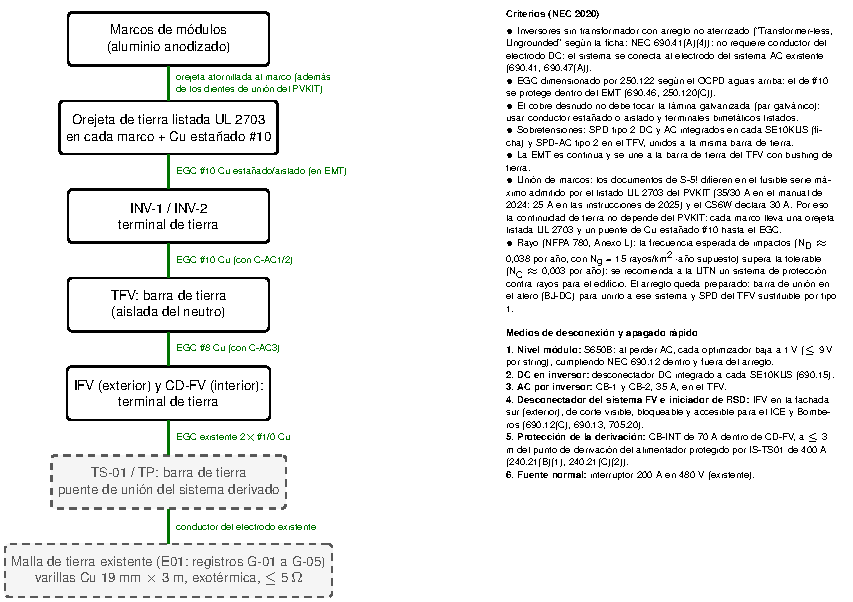
\includegraphics[height=138mm]{detalle_tierra_sa.pdf}};
% ---------------- Pruebas ----------------
\node[anchor=north west,font=\fontsize{9}{11}\selectfont\bfseries] at (15,128) {PRUEBAS DE PUESTA EN MARCHA (IEC 62446-1:2016+A1:2018)};
\node[anchor=north west,font=\fontsize{7.2}{9}\selectfont,align=left,text width=225mm] at (15,122) {%
1. Inspección visual: listados, torques, rótulos, canalizaciones, orejetas de tierra y unión equipotencial del arreglo (UL 2703).\\
2. Continuidad de EGC y unión equipotencial: marcos, rack, EMT, inversores, TFV, IFV, CD-FV hasta la barra de tierra de TS-01/TP.\\
3. Polaridad y tensión de cada string con el sistema en modo seguro (9 V esperados con 9 optimizadores a 1 V).\\
4. Resistencia de aislamiento de los circuitos DC (inversor y megóhmetro) y de los circuitos AC nuevos.\\
5. Prueba funcional de apagado rápido: abrir IFV y verificar $\le$ 30 V fuera del arreglo y $\le$ 80 V dentro en $\le$ 30 s (NEC 690.12).\\
6. Prueba de anti-isla coordinada con el ATS: abrir la fuente normal y verificar el cese de inyección en $\le$ 2 s, antes de la transferencia (retardo del ATS $\ge$ 3 s), y la reconexión retardada al volver la red.\\
7. Medición de la resistencia de la malla existente ($\le$ 5 $\Omega$, E02--E06) y termografía de bornes a plena carga.\\
8. Registro de los ajustes de protección del inversor (IEEE 1547-2018, perfil acordado con el ICE) y entrega de la documentación \emph{as-built}.};
% ---------------- Columna derecha: rótulos ----------------
\node[anchor=north west,font=\fontsize{9}{11}\selectfont\bfseries] at (252,283) {CUADRO DE RÓTULOS};
\node[anchor=north west,font=\fontsize{5.6}{6.8}\selectfont] at (252,277) {%
\setlength{\tabcolsep}{2pt}\begin{tabular}{@{}p{24mm}p{88mm}p{38mm}@{}}
\textbf{Ubicación} & \textbf{Texto (resumido)} & \textbf{Requisito}\\\hline
Nicho 480 V, ATS, TP & ADVERTENCIA: ESTE EDIFICIO TIENE TRES FUENTES DE ENERGÍA: RED ICE, GENERADOR Y SISTEMA FV. Ubicación de los desconectadores: \ldots & NEC 705.10 (directorio)\\
Servicio / cuarto eléctrico & SISTEMA FV EQUIPADO CON APAGADO RÁPIDO. COLOQUE EL INTERRUPTOR IFV EN ``OFF'' PARA APAGAR EL SISTEMA FV Y REDUCIR EL RIESGO DE CHOQUE EN EL ARREGLO (con esquema) & NEC 690.56(C)(1)\\
IFV & INTERRUPTOR DE APAGADO RÁPIDO DEL SISTEMA FV (blanco sobre rojo, reflectivo) / DESCONECTADOR DEL SISTEMA FV / ADVERTENCIA: LOS TERMINALES DE LÍNEA Y CARGA PUEDEN ESTAR ENERGIZADOS EN POSICIÓN ABIERTA & NEC 690.12(C), 690.13(B), 690.56(C)(2), 705.20\\
IFV, CD-FV & FUENTE DE POTENCIA FV: CORRIENTE AC NOMINAL 55,6 A; TENSIÓN AC NOMINAL 208 V & NEC 690.54\\
TFV & EQUIPO ALIMENTADO POR MÚLTIPLES FUENTES: LA SUMA DE LOS DISPOSITIVOS DE SOBRECORRIENTE (EXCLUIDO EL QUE PROTEGE LAS BARRAS) NO DEBE EXCEDER LA CAPACIDAD DE LAS BARRAS & NEC 705.12(B)(3)(3)\\
Inversores (DC) & FUENTE FV -- TENSIÓN DC MÁXIMA 600 V & NEC 690.53\\
CD-FV, TFV & ADVERTENCIA: FUENTE DUAL -- PUEDE ESTAR ENERGIZADO DESDE AMBOS LADOS & NEC 705.12(C)\\
EMT DC (cada $\le$ 3 m, en curvas y pasos) & CIRCUITO DC SOLAR FV (reflectivo, blanco sobre rojo, $\ge$ 9,5 mm) & NEC 690.31(D)(2)\\
Tableros nuevos & ADVERTENCIA: RIESGO DE ARCO ELÉCTRICO & NEC 110.16, 110.21(B)\\
Acceso a la cubierta & CUBIERTA CON PANELES SOLARES -- USE LOS PASILLOS SEÑALADOS & NFPA 1 \S 11.12\\\hline
\end{tabular}};
\node[anchor=north west,font=\fontsize{5.8}{7.2}\selectfont,align=left,text width=152mm] at (252,196) {%
Rótulos permanentes, resistentes a UV y a la intemperie (NEC 110.21(B)). Interruptor de apagado rápido: reflectivo, letras blancas sobre rojo de al menos 9,5 mm (690.56(C)(2)). Rótulo de edificio con apagado rápido: título negro sobre amarillo de al menos 9,5 mm y resto negro sobre blanco de al menos 4,8 mm, con esquema del arreglo (690.56(C)(1)).};
\node[anchor=north west,font=\fontsize{9}{11}\selectfont\bfseries] at (252,180) {SECUENCIA DE DESCONEXIÓN DE EMERGENCIA};
\node[anchor=north west,font=\fontsize{6}{7.4}\selectfont,align=left,text width=152mm] at (252,174) {%
1. Abrir el \textbf{IFV} (fachada sur, exterior): los inversores cesan la inyección y los optimizadores llevan el arreglo a 1 V por módulo.\\
2. Si se requiere aislar el edificio: abrir el interruptor de 200 A en el nicho del transformador ICE y bloquear el ATS en posición ``OFF'' o el generador.\\
3. Para mantenimiento de un inversor: abrir CB-1 o CB-2 en el TFV y el desconectador DC integrado del inversor; esperar 5 min antes de abrir la tapa.\\
4. Aplicar bloqueo y etiquetado (LOTO) en IFV, CB-1/CB-2 y CB-INT de CD-FV.};
\node[anchor=north west,font=\fontsize{9}{11}\selectfont\bfseries] at (252,138) {CONDUCTORES DE PUESTA A TIERRA};
\node[anchor=north west,font=\fontsize{5.8}{7}\selectfont] at (252,132) {%
\setlength{\tabcolsep}{2pt}\begin{tabular}{@{}lllp{60mm}@{}}
\textbf{Tramo} & \textbf{OCPD} & \textbf{EGC} & \textbf{Criterio}\\\hline
Marcos $\rightarrow$ EGC & -- & \#10 Cu est. & Orejeta UL 2703; puente estañado\\
Arreglo $\rightarrow$ INV & -- & \#10 Cu & 690.45/250.122; en EMT (690.46)\\
INV $\rightarrow$ TFV & 35 A & \#10 Cu & 250.122 (hasta 60 A)\\
TFV $\rightarrow$ IFV $\rightarrow$ CD-FV & 70 A & \#8 Cu & 250.122 (hasta 100 A)\\
CD-FV $\rightarrow$ barra TS-01/TP & -- & existente & 2 $\times$ \#1/0 Cu (E07)\\\hline
\end{tabular}};
% Leyenda
\node[anchor=north west,font=\fontsize{9}{11}\selectfont\bfseries] at (252,104) {LEYENDA};
\begin{scope}[shift={(252,92)},font=\fontsize{6}{7.4}\selectfont]
\draw[thick,rounded corners=1pt] (0,4) rectangle (12,8); \node[anchor=west] at (14,6) {Equipo o elemento nuevo};
\draw[thick,dashed,gray!70!black,fill=gray!8,rounded corners=1pt] (0,-1) rectangle (12,3); \node[anchor=west] at (14,1) {Equipo o elemento existente (E01, E07)};
\draw[very thick,green!50!black] (0,-5) -- (12,-5); \node[anchor=west] at (14,-5) {Conductor de puesta a tierra / unión equipotencial (calibre indicado)};
\node[anchor=north west,text width=150mm,align=left] at (0,-8.5) {IFV = desconectador FV e iniciador RSD; TFV = tablero FV; CD-FV = caja de derivación; CB = interruptor; RSD = apagado rápido; EGC = conductor de tierra de equipos.};
\end{scope}
\cajetin{FV-04}{Puesta a tierra, equipotencialización, medios de}{desconexión, rotulación y pruebas}{Sin escala}{5 de 5}
\end{tikzpicture}
\end{document}
